% ---- closed --------

\begin{figure}[!htb]
    \centering
    \begin{minipage}[b]{0.45\textwidth}
        \centering
        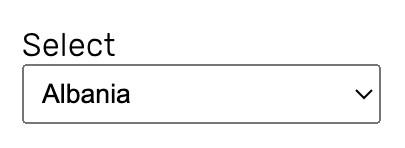
\includegraphics[width=0.8\textwidth]{closed.osx.chrome.png}
        \caption{Geschlossenes Select auf OSX Chrome}
        \label{img:closedOsxChromeSelect}
    \end{minipage}
    \hfill
    \begin{minipage}[b]{0.45\textwidth}
        \centering
        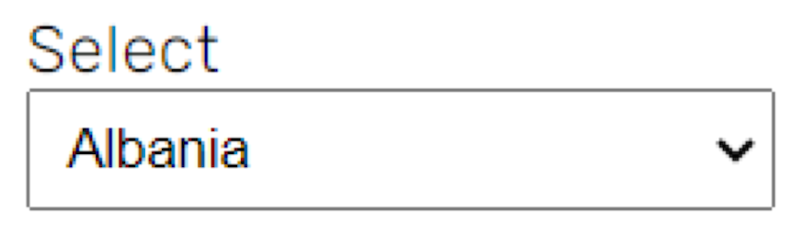
\includegraphics[width=0.8\textwidth]{closed.win.chrome.png}
        \caption{Geschlossenes Select auf Windows Chrome}
        \label{img:closedWinChromeSelect}
    \end{minipage}
\end{figure}

\begin{figure}[!htb]
    \centering
    \begin{minipage}[b]{0.45\textwidth}
        \centering
        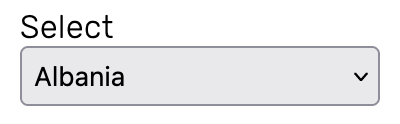
\includegraphics[width=0.8\textwidth]{closed.osx.firefox.png}
        \caption{Geschlossenes Select auf OSX Firefox}
        \label{img:closedOsxFirefoxSelect}
    \end{minipage}
    \hfill
    \begin{minipage}[b]{0.45\textwidth}
        \centering
        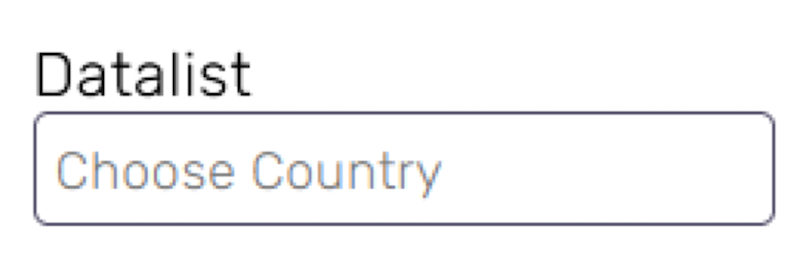
\includegraphics[width=0.8\textwidth]{closed.win.firefox.png}
        \caption{Geschlossenes Select auf Windows Firefox}
        \label{img:closedWinFirefoxSelect}
    \end{minipage}
\end{figure}

\begin{figure}[!htb]
    \centering
    \begin{minipage}[b]{0.45\textwidth}
        \centering
        
\includegraphics[width=0.8\textwidth]{closed.osx.safari.png}
        \caption{Geschlossenes Select auf OSX Safari}
        \label{img:closedOsxSafariSelect}
    \end{minipage}
    \hfill
    \begin{minipage}[b]{0.45\textwidth}
        \centering
        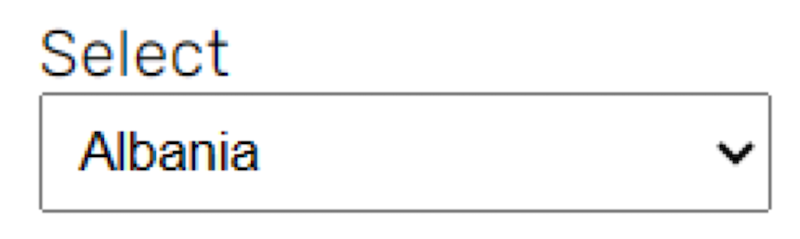
\includegraphics[width=0.8\textwidth]{closed.win.edge.png}
        \caption{Geschlossenes Select auf Windows Edge}
        \label{img:closedWinEdgeSelect}
    \end{minipage}
\end{figure}

% ---- opened --------

\begin{figure}[!htb]
    \centering
    \begin{minipage}[b]{0.28\textwidth}
        \centering
        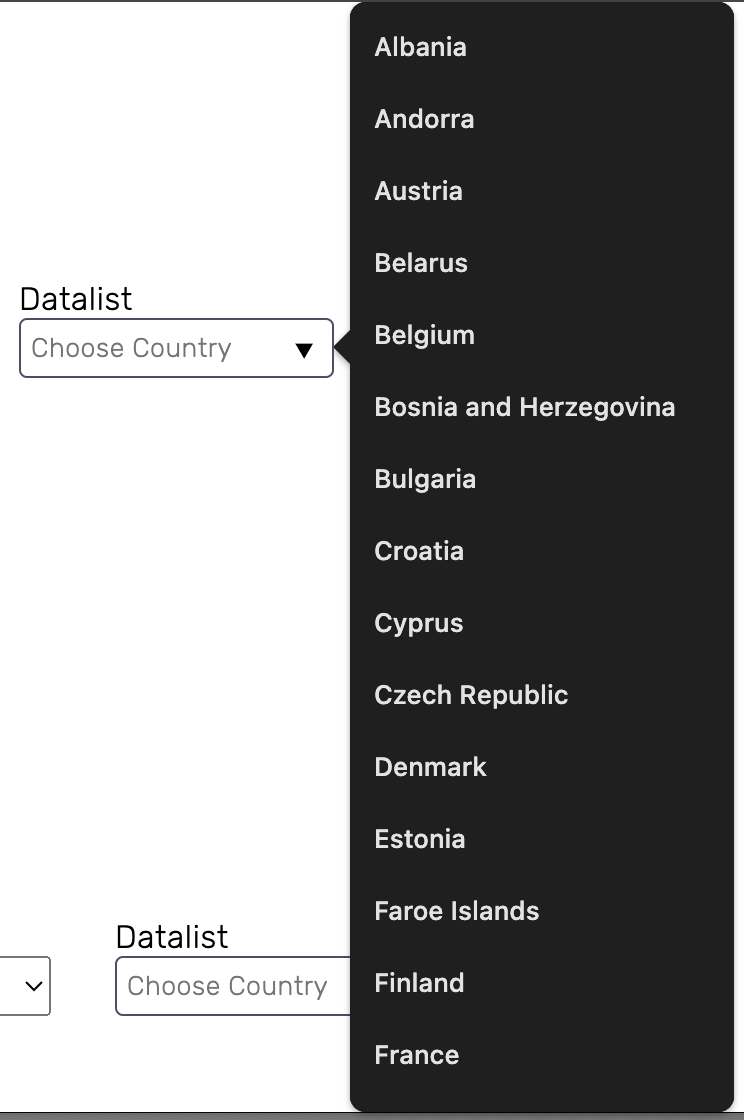
\includegraphics[width=0.55\textwidth]{opened.osx.chrome.png}
        \caption{Offenes Select auf OSX Chrome}
        \label{img:openedOsxChromeSelect}
    \end{minipage}
    \hfill
    \begin{minipage}[b]{0.28\textwidth}
        \centering
        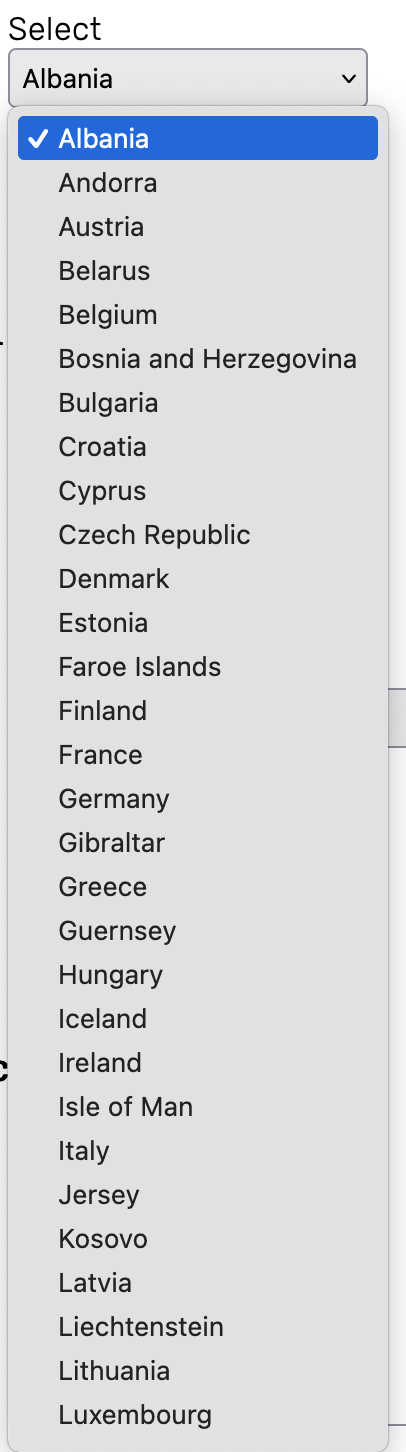
\includegraphics[width=0.5\textwidth]{opened.osx.firefox.png}
        \caption{Offenes Select auf OSX Firefox}
        \label{img:openedOsxFirefoxSelect}
    \end{minipage}
    \hfill
    \begin{minipage}[b]{0.28\textwidth}
        \centering
        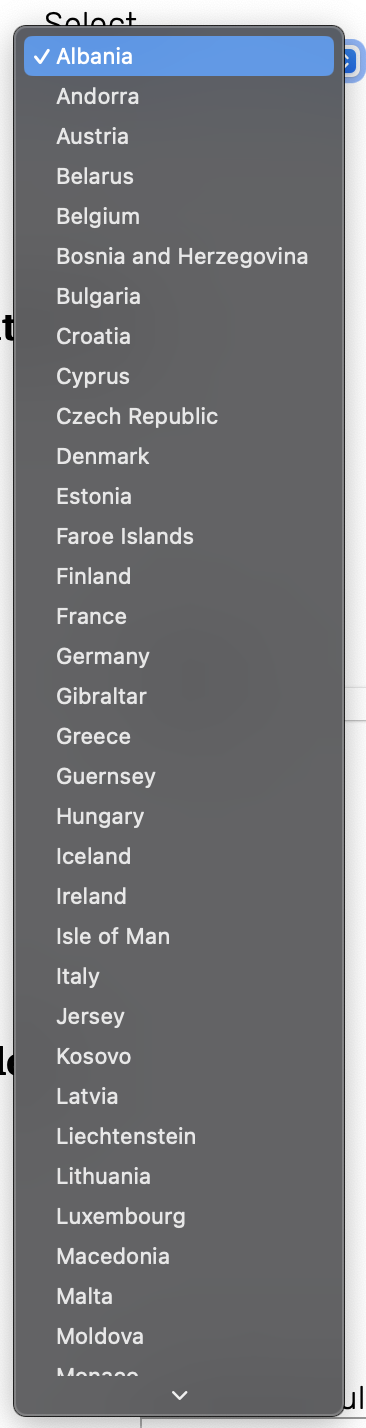
\includegraphics[width=0.45\textwidth]{opened.osx.safari.png}
        \caption{Offenes Select auf OSX Safari}
        \label{img:openedOsxSafariSelect}
    \end{minipage}
\end{figure}

\begin{figure}[!htb]
    \centering
    \begin{minipage}[b]{0.28\textwidth}
        \centering
        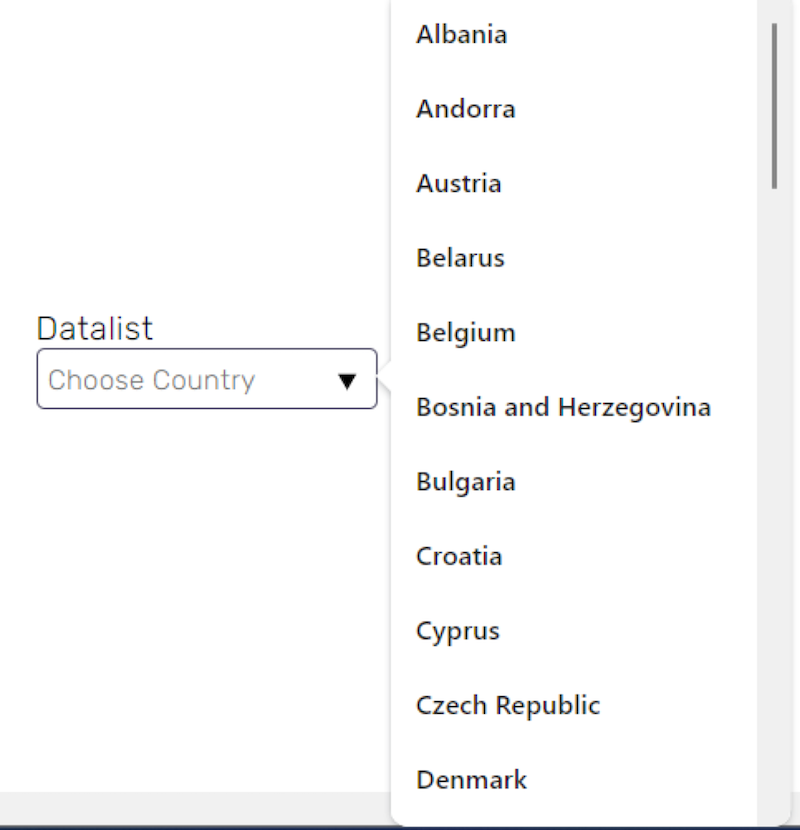
\includegraphics[width=0.65\textwidth]{opened.win.chrome.png}
        \caption{Offenes Select auf Windows Chrome}
        \label{img:openedWinChromeSelect}
    \end{minipage}
    \hfill
    \begin{minipage}[b]{0.28\textwidth}
        \centering
        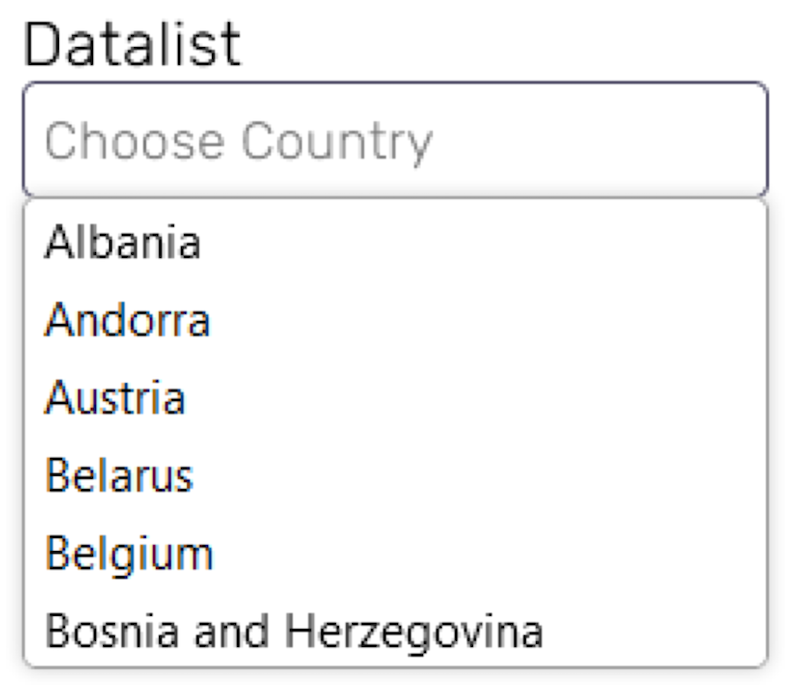
\includegraphics[width=0.6\textwidth]{opened.win.firefox.png}
        \caption{Offenes Select auf Windows Firefox}
        \label{img:openedWinFirefoxSelect}
    \end{minipage}
    \hfill
    \begin{minipage}[b]{0.28\textwidth}
        \centering
        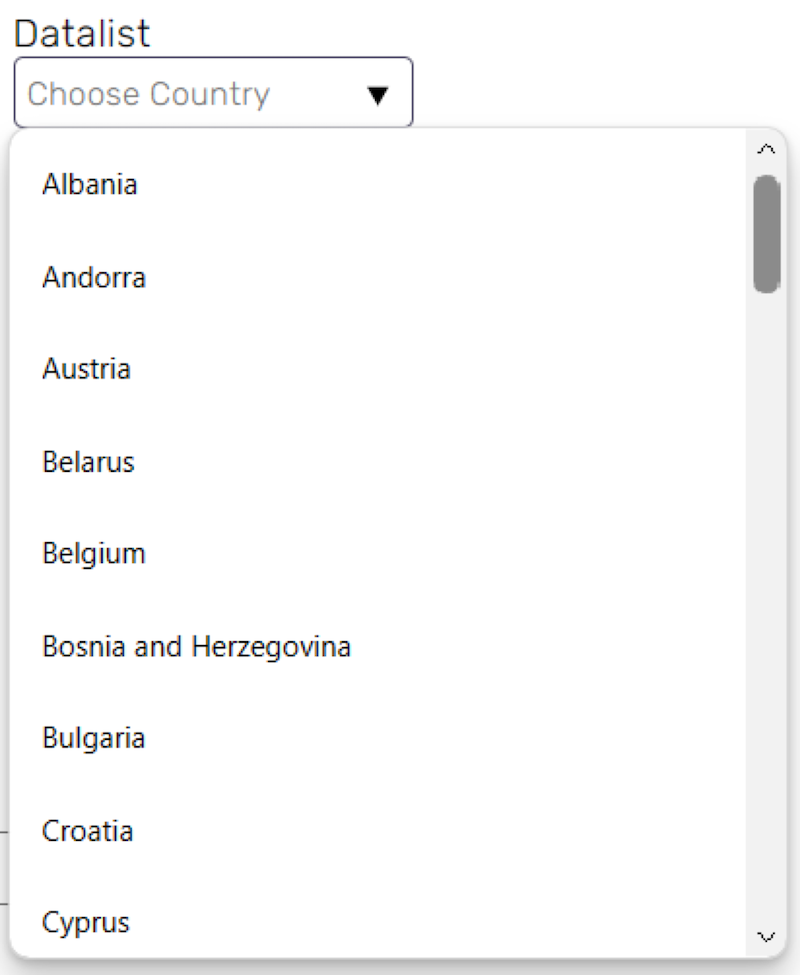
\includegraphics[width=0.65\textwidth]{opened.win.edge.png}
        \caption{Offenes Select auf Windows Edge}
        \label{img:openedWinEdgeSelect}
    \end{minipage}
\end{figure}

% ---- mobile --------

\begin{figure}[!htb]
    \centering
    \begin{minipage}[b]{0.45\textwidth}
        \centering
        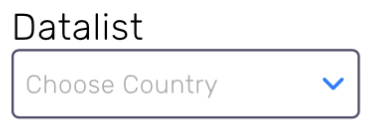
\includegraphics[width=0.8\textwidth]{closed.ios.safari.png}
        \caption{Geschlossenes Select auf iOS Safari}
        \label{img:closedIosSafariSelect}
    \end{minipage}
    \hfill
    \begin{minipage}[b]{0.45\textwidth}
        \centering
        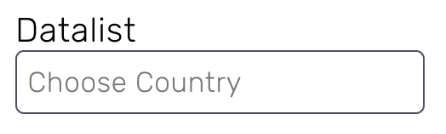
\includegraphics[width=0.8\textwidth]{closed.android.firefox.png}
        \caption{Geschlossenes Select auf Android Firefox}
        \label{img:closedAndroidFirefoxSelect}
    \end{minipage}
\end{figure}

\begin{figure}[!htb]
    \centering
    \begin{minipage}[b]{0.45\textwidth}
        \centering
        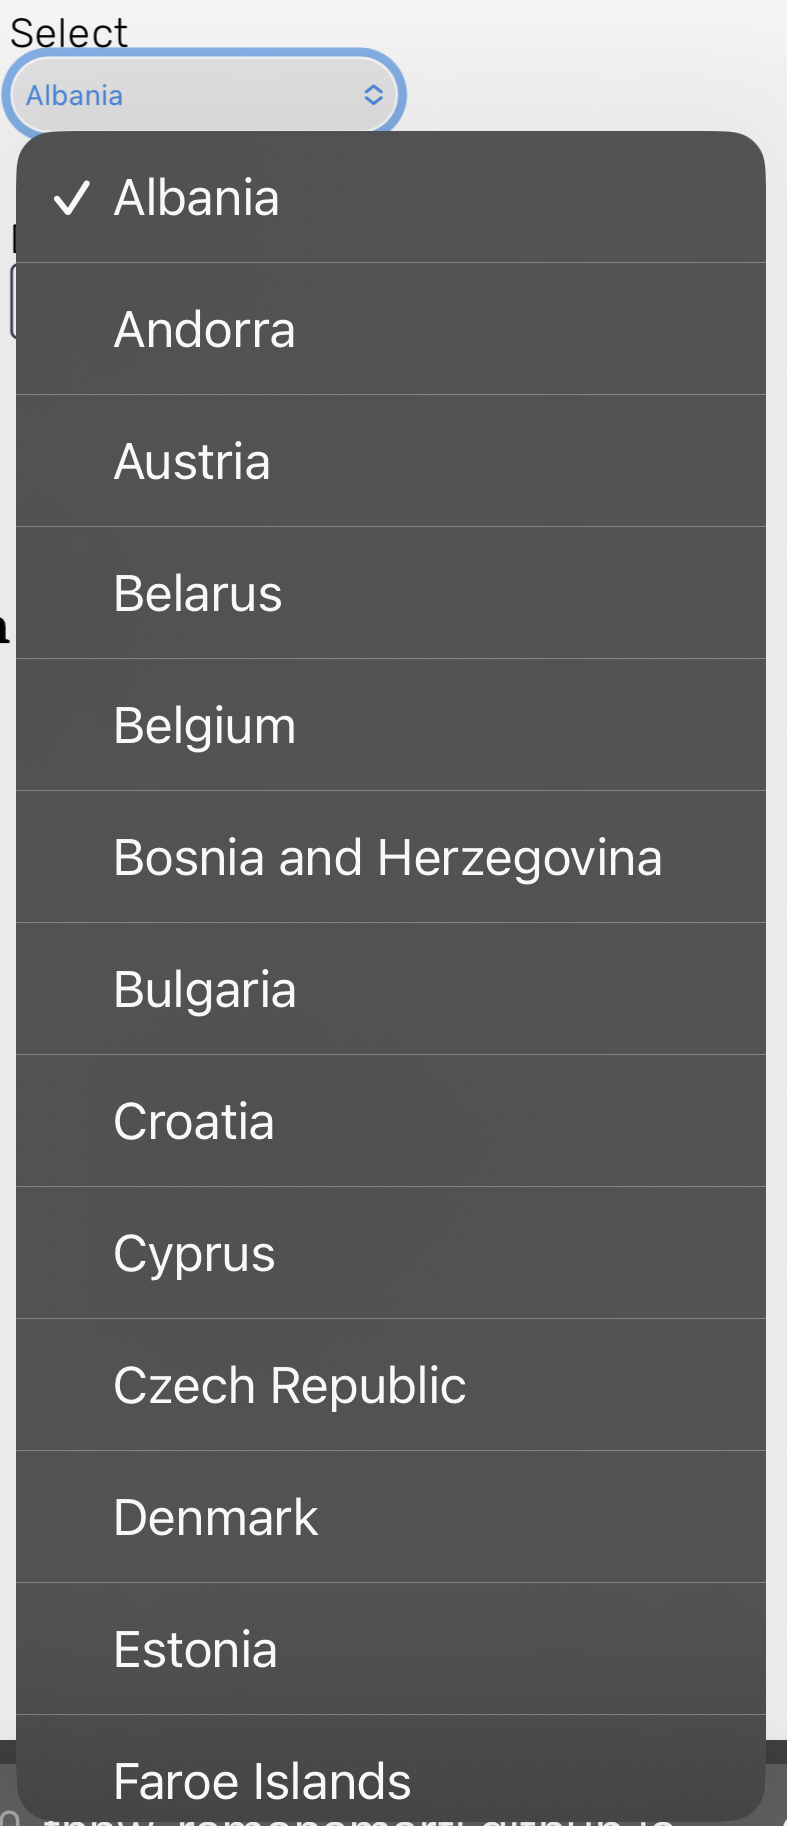
\includegraphics[width=0.8\textwidth]{opened.ios.safari.png}
        \caption{Offenes Select auf iOS Safari}
        \label{img:openedIosSafariSelect}
    \end{minipage}
    \hfill
    \begin{minipage}[b]{0.45\textwidth}
        \centering
        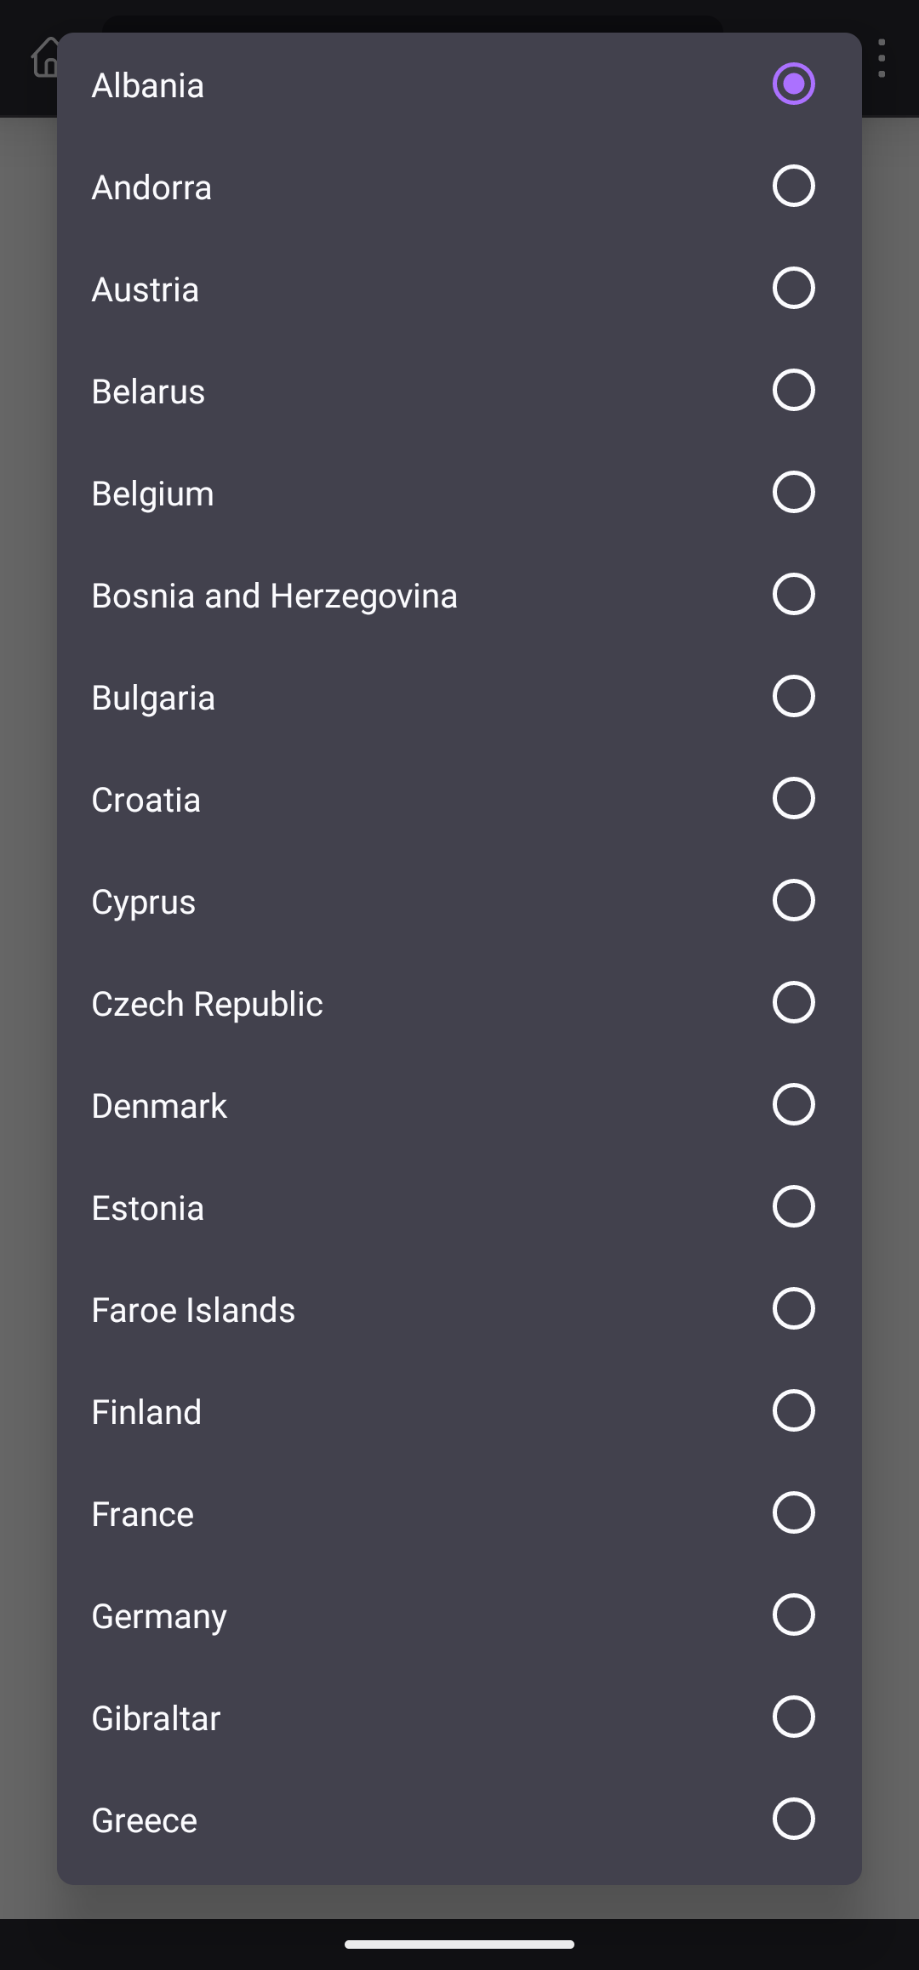
\includegraphics[width=0.8\textwidth]{opened.android.firefox.png}
        \caption{Offenes Select auf Android Firefox}
        \label{img:openedAndroidFirefoxSelect}
    \end{minipage}
\end{figure}

% ---- disabled --------

\begin{figure}[!htb]
    \centering
    \begin{minipage}[b]{0.28\textwidth}
        \centering
        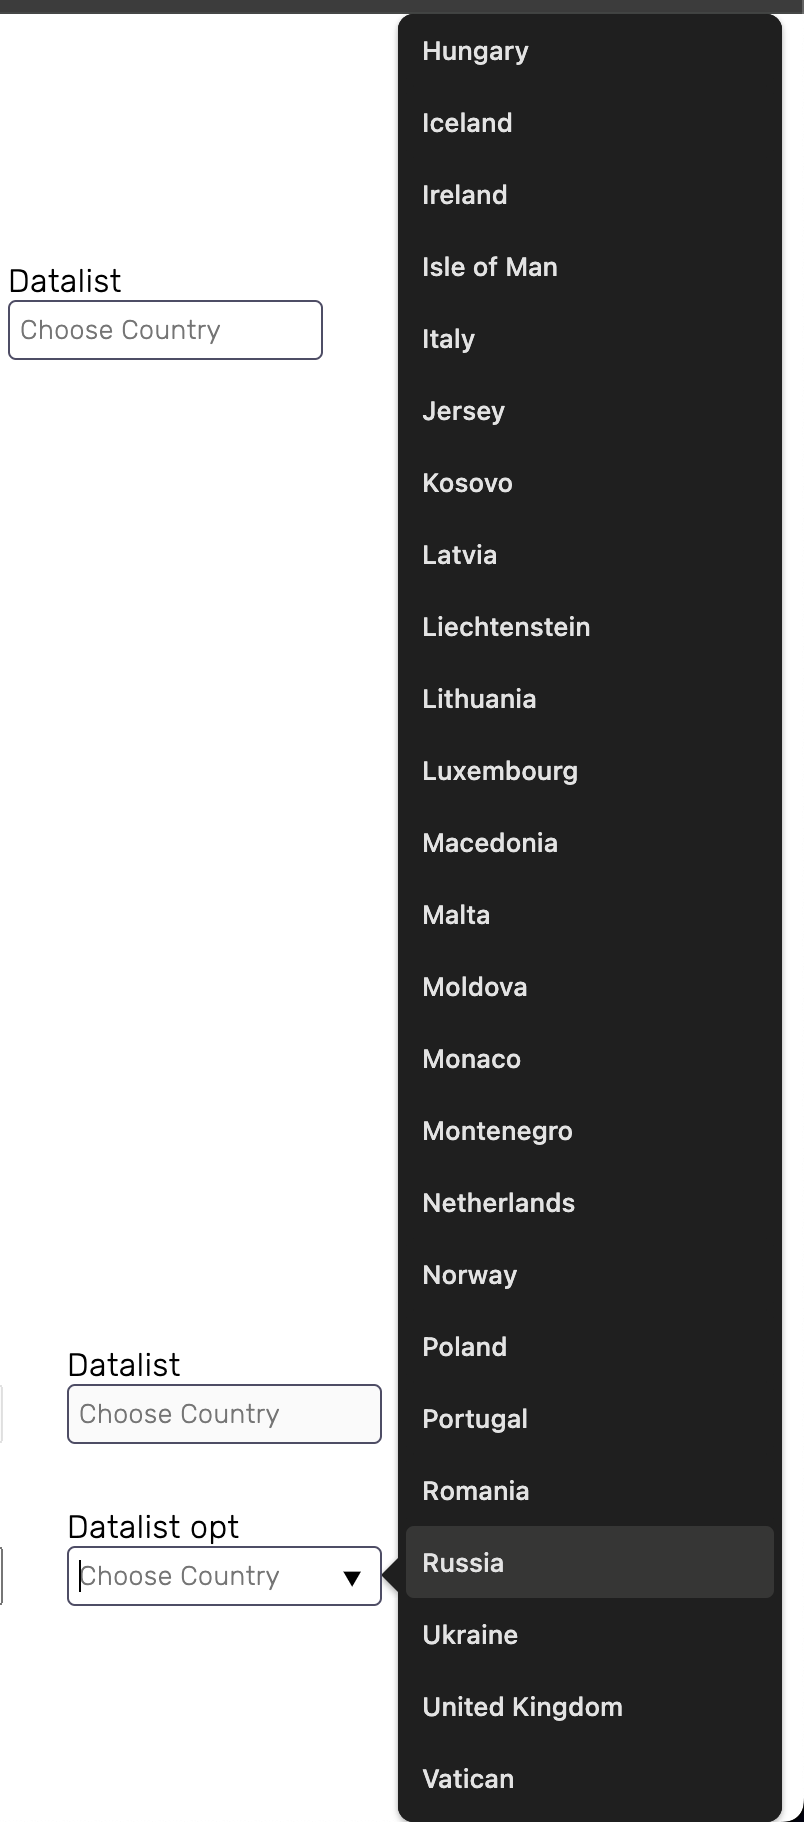
\includegraphics[width=0.95\textwidth]{disabled.osx.chrome.png}
        \caption{Disabled Select auf OSX Chrome}
        \label{img:disabledOsxChromeSelect}
    \end{minipage}
    \hfill
    \begin{minipage}[b]{0.28\textwidth}
        \centering
        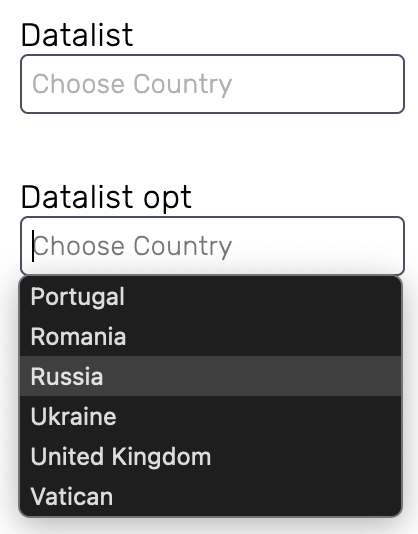
\includegraphics[width=0.65\textwidth]{disabled.osx.firefox.png}
        \caption{Disabled Select auf OSX Firefox}
        \label{img:disabledOsxFirefoxSelect}
    \end{minipage}
    \hfill
    \begin{minipage}[b]{0.28\textwidth}
        \centering
        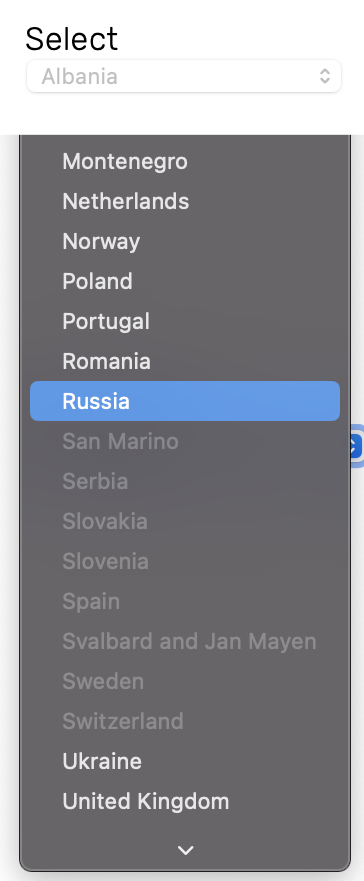
\includegraphics[width=0.75\textwidth]{disabled.osx.safari.png}
        \caption{Disabled Select auf OSX Safari}
        \label{img:disabledOsxSafariSelect}
    \end{minipage}
\end{figure}

\begin{figure}[!htb]
    \centering
    \begin{minipage}[b]{0.28\textwidth}
        \centering
        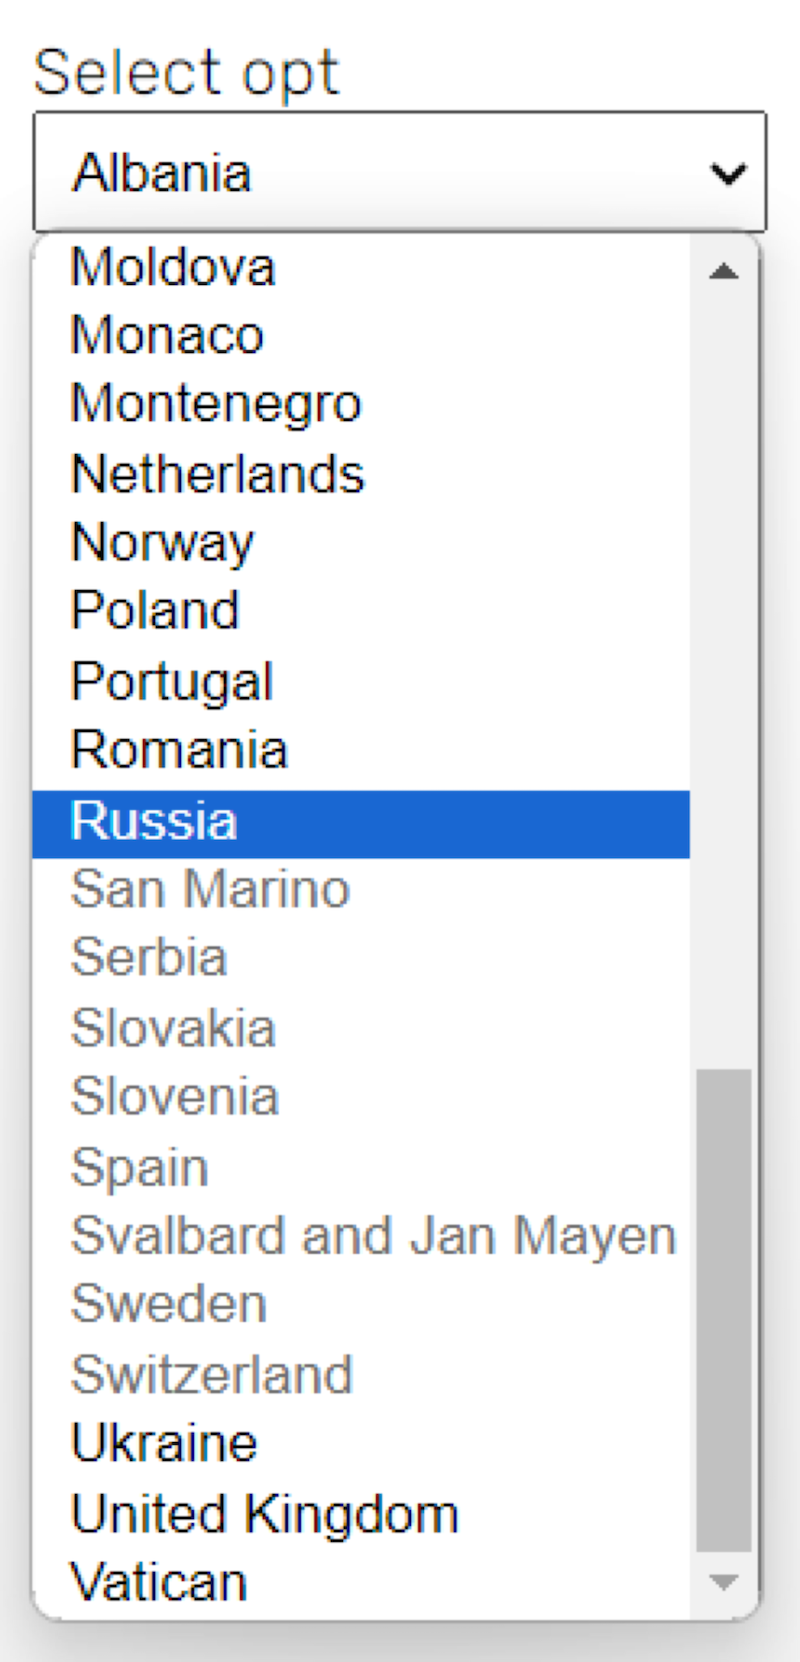
\includegraphics[width=0.9\textwidth]{disabled.win.chrome.png}
        \caption{Disabled Select auf Windows Chrome}
        \label{img:disabledWinChromeSelect}
    \end{minipage}
    \hfill
    \begin{minipage}[b]{0.28\textwidth}
        \centering
        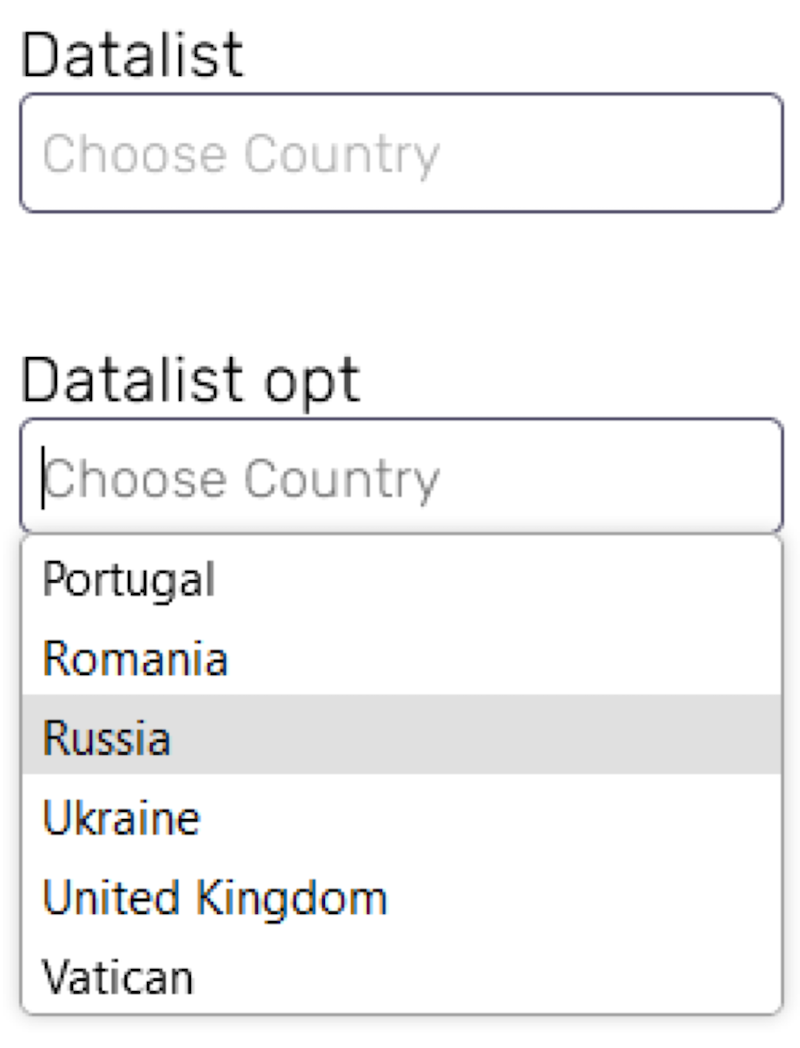
\includegraphics[width=0.6\textwidth]{disabled.win.firefox.png}
        \caption{Disabled Select auf Windows Firefox}
        \label{img:disabledWinFirefoxSelect}
    \end{minipage}
    \hfill
    \begin{minipage}[b]{0.28\textwidth}
        \centering
        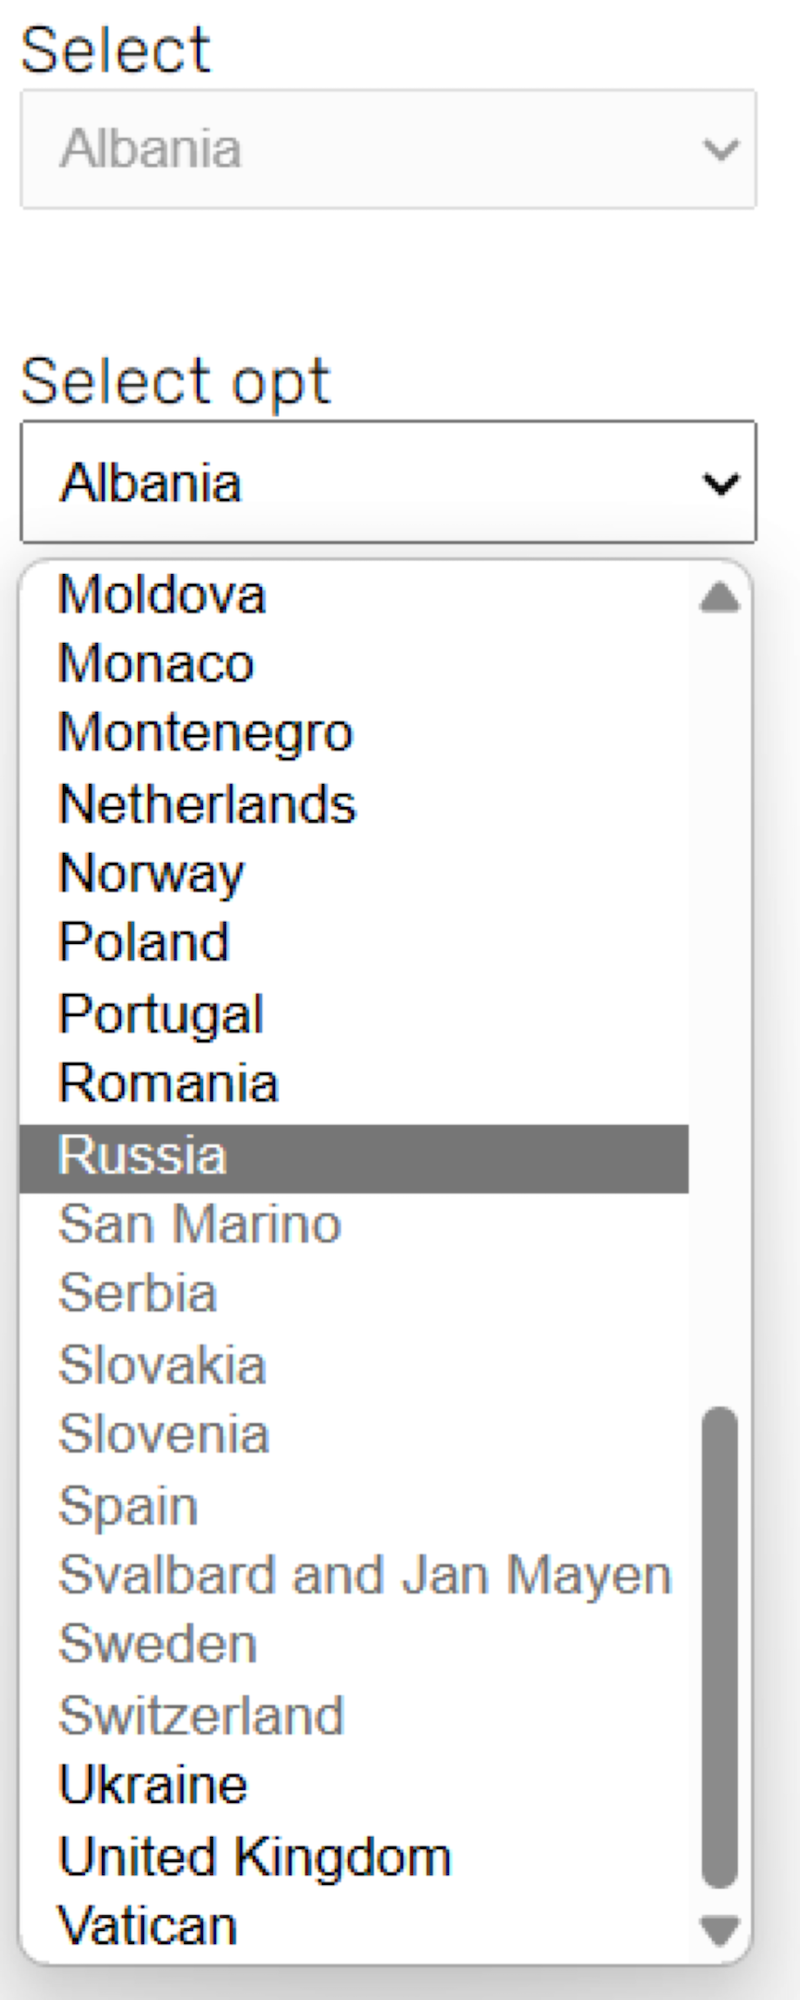
\includegraphics[width=0.85\textwidth]{disabled.win.edge.png}
        \caption{Disabled Select auf Windows Edge}
        \label{img:disabledWinEdgeSelect}
    \end{minipage}
\end{figure}

% ---- multiple --------

\begin{figure}[!htb]
    \centering
    \begin{minipage}[b]{0.45\textwidth}
        \centering
        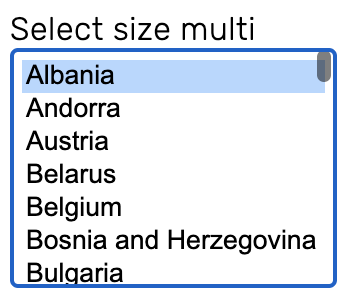
\includegraphics[width=0.8\textwidth]{multi.osx.chrome.png}
        \caption{Multi-Select auf OSX Chrome}
        \label{img:multiOsxChromeSelect}
    \end{minipage}
    \hfill
    \begin{minipage}[b]{0.45\textwidth}
        \centering
        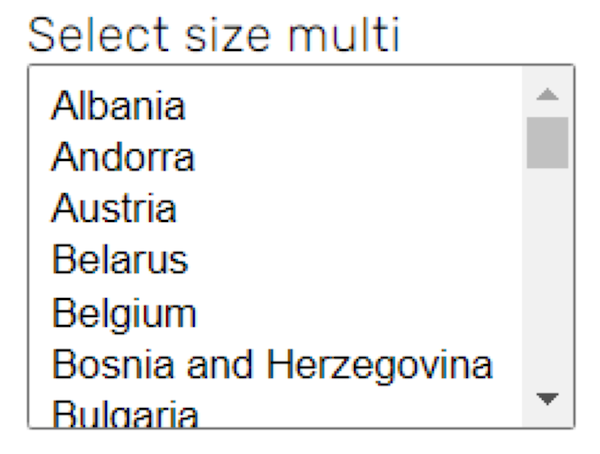
\includegraphics[width=0.8\textwidth]{multi.win.chrome.png}
        \caption{Multi-Select auf Windows Chrome}
        \label{img:multiWinChromeSelect}
    \end{minipage}
\end{figure}

\begin{figure}[!htb]
    \centering
    \begin{minipage}[b]{0.45\textwidth}
        \centering
        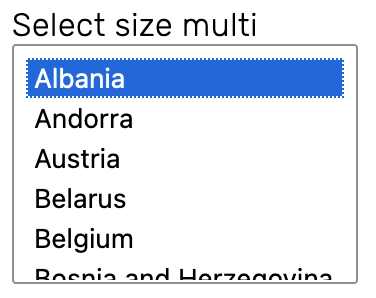
\includegraphics[width=0.8\textwidth]{multi.osx.firefox.png}
        \caption{Multi-Select auf OSX Firefox}
        \label{img:multiOsxFirefoxSelect}
    \end{minipage}
    \hfill
    \begin{minipage}[b]{0.45\textwidth}
        \centering
        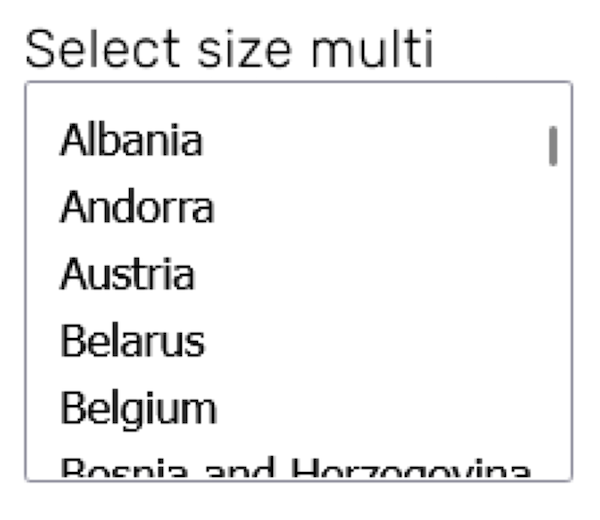
\includegraphics[width=0.8\textwidth]{multi.win.firefox.png}
        \caption{Multi-Select auf Windows Firefox}
        \label{img:multiWinFirefoxSelect}
    \end{minipage}
\end{figure}

\begin{figure}[!htb]
    \centering
    \begin{minipage}[b]{0.45\textwidth}
        \centering
        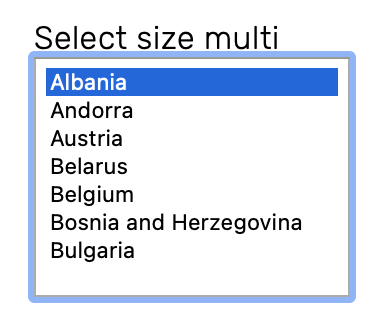
\includegraphics[width=0.8\textwidth]{multi.osx.safari.png}
        \caption{Multi-Select auf OSX Safari}
        \label{img:multiOsxSafariSelect}
    \end{minipage}
    \hfill
    \begin{minipage}[b]{0.45\textwidth}
        \centering
        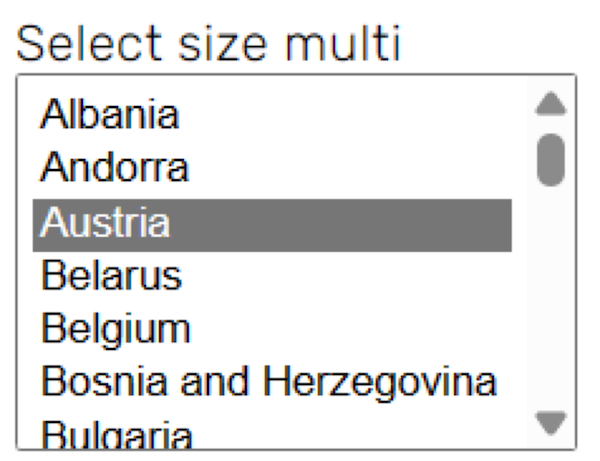
\includegraphics[width=0.8\textwidth]{multi.win.edge.png}
        \caption{Multi-Select auf Windows Edge}
        \label{img:multiWinEdgeSelect}
    \end{minipage}
\end{figure}

% ---- optgroup --------

\begin{figure}[!htb]
    \centering
    \begin{minipage}[b]{0.28\textwidth}
        \centering
        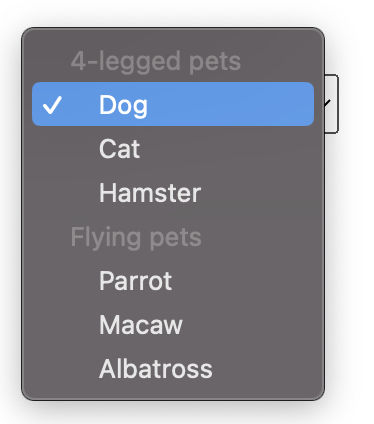
\includegraphics[width=0.9\textwidth]{optgroup.osx.chrome.png}
        \caption{Select mit Optgroups auf OSX Chrome}
        \label{img:optgroupOsxChromeSelect}
    \end{minipage}
    \hfill
    \begin{minipage}[b]{0.28\textwidth}
        \centering
        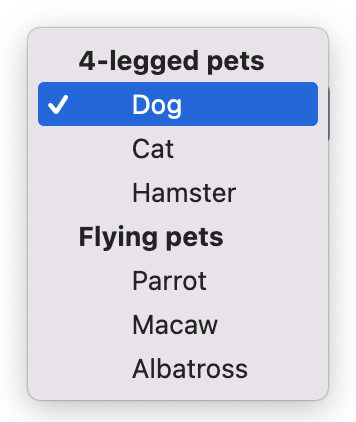
\includegraphics[width=0.9\textwidth]{optgroup.osx.firefox.png}
        \caption{Select mit Optgroups auf OSX Firefox}
        \label{img:optgroupOsxFirefoxSelect}
    \end{minipage}
    \hfill
    \begin{minipage}[b]{0.28\textwidth}
        \centering
        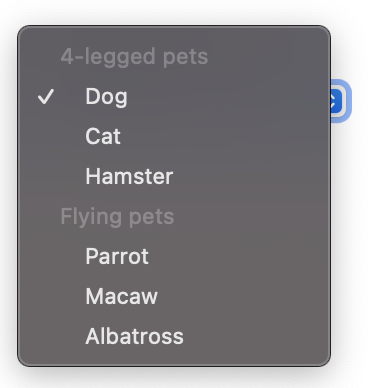
\includegraphics[width=0.9\textwidth]{optgroup.osx.safari.png}
        \caption{Select mit Optgroups auf OSX Safari}
        \label{img:optgroupOsxSafariSelect}
    \end{minipage}
\end{figure}

\begin{figure}[!htb]
    \centering
    \begin{minipage}[b]{0.28\textwidth}
        \centering
        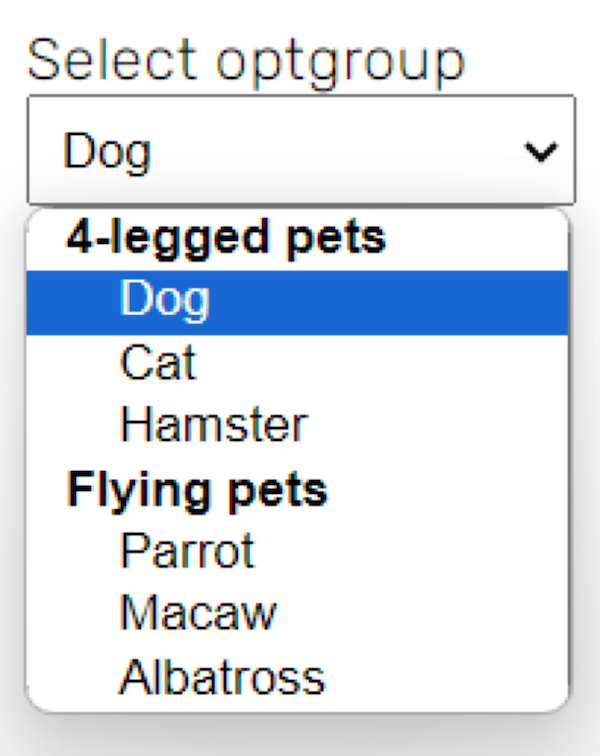
\includegraphics[width=0.9\textwidth]{optgroup.win.chrome.png}
        \caption{Select mit Optgroups auf Windows Chrome}
        \label{img:optgroupWinChromeSelect}
    \end{minipage}
    \hfill
    \begin{minipage}[b]{0.28\textwidth}
        \centering
        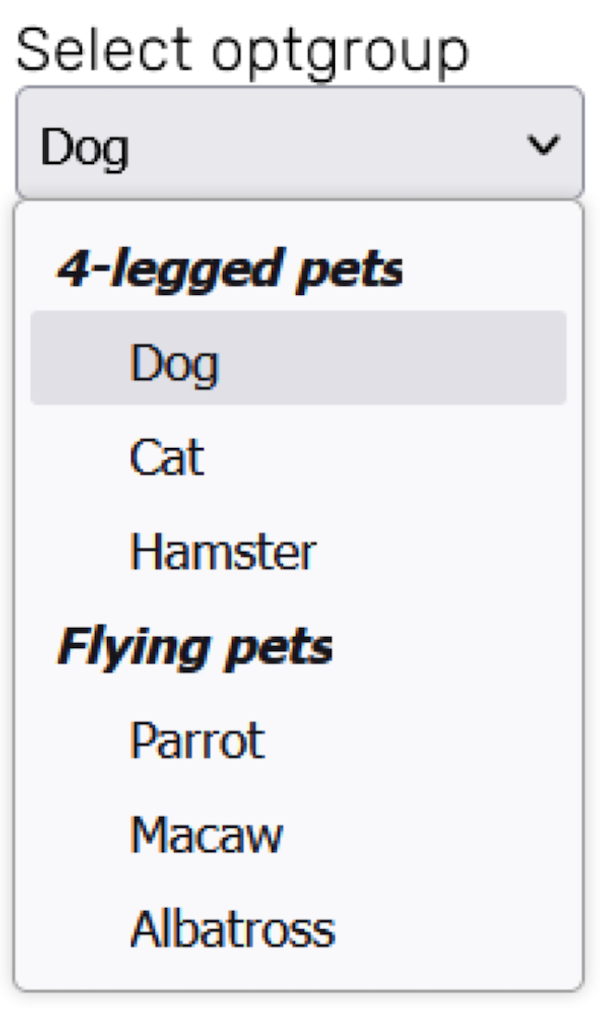
\includegraphics[width=0.7\textwidth]{optgroup.win.firefox.png}
        \caption{Select mit Optgroups auf Windows Firefox}
        \label{img:optgroupWinFirefoxSelect}
    \end{minipage}
    \hfill
    \begin{minipage}[b]{0.28\textwidth}
        \centering
        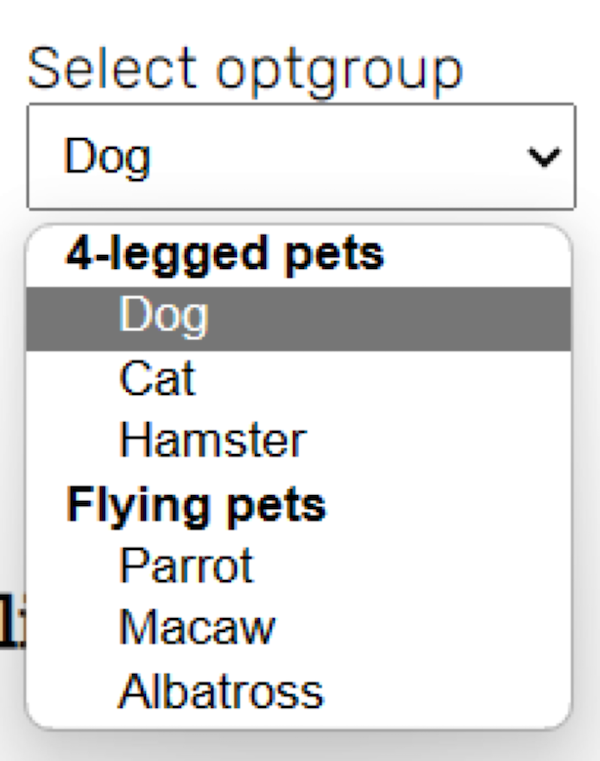
\includegraphics[width=0.9\textwidth]{optgroup.win.edge.png}
        \caption{Select mit Optgroups auf Windows Edge}
        \label{img:optgroupWinEdgeSelect}
    \end{minipage}
\end{figure}
